% https://tex.stackexchange.com/a/762541
\documentclass[tikz,border=5pt]{standalone}
\usepackage{fourier}
\usetikzlibrary{bending,decorations.pathmorphing}
\begin{document}
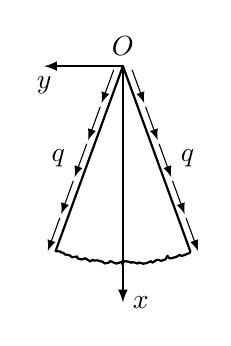
\begin{tikzpicture}[>=latex,line join=round,line cap=round]
\draw[semithick,->] (0,0) -- (-1,0) node[below] {$y$};
\draw[semithick,->] (0,0) -- (0,-3) node[right] {$x$};
\draw[thick] (-110:2.5) -- node[left=5pt] {$q$} (0,0) node[above] {$O$} -- node[right=5pt] {$q$} (-70:2.5);
\def\tmp{\fpeval{2.5*sind(20)}}
\draw[thick, decorate, decoration={random steps, segment length=1pt, amplitude=.75pt}] (-110:2.5) arc[start angle=-110, end angle=-70, radius=2.5];
\foreach \i in {1,...,5}{
    \draw[->,shorten <=1.5pt] (-.1,0) ++(-110:{(\i-1)*0.5}) -- ++(-110:0.5);
    \draw[->,shorten <=1.5pt] (+.1,0) ++(-70:{(\i-1)*0.5}) -- ++(-70:0.5);
}
\end{tikzpicture}
\end{document}